In general a slam output will give either a topological map or an Occupancy Grid\\

\subsection{Topological Map}

If the algorithm for the SLAM uses landmarks there is chance that it uses a topological map. This type of map will put in relation different landmarks as a graph, the nodes will be the landmarks and the arc can be the path, the distance between the landmarks, for example an underground map is a topological map with stations such as the landmarks and relations are the connections between the stations:\\

\begin{figure}[H]
\centering
    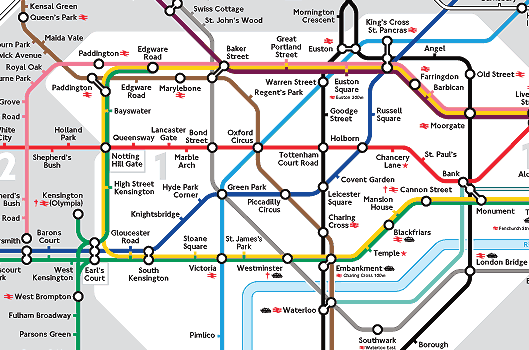
\includegraphics[scale=0.3]{topo.png} 
    \caption{Example of a topological map.}
    \label{fig:topoExample}
\end{figure}

This type of map will be made when sensors can distinguish features in the environment. This type of map has a higher abstraction level, it does not know the metrics of the environment but it can consider objects in it:

\begin{figure}[H]
\centering
    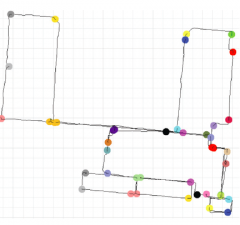
\includegraphics[scale=0.6]{topo2.png} 
    \caption{Example of a SLAM topological map \cite{Ranganathan10ijrr}.}
    \label{fig:topo2Example}
\end{figure}

 In figure~\ref{fig:topo2Example} the landmarks are corners and intersections. 

\subsection{Occupancy Grid}

An occupancy grid will represent the continuous space divided in a 2 or 3D grid where each square or box contains the probability of being occupied, in figure 3 the squares are in a trinary state (empty , occupied or unknown):


\begin{figure}[H]
\centering
    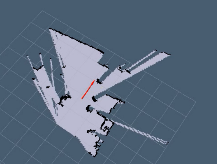
\includegraphics[scale=2.2]{occupGrid.png} 
    \caption{2D Occupancy Grid of the Robotic Club in ENSTA Bretagne with Hector Slam~\cite{kohlbrecher2011flexible}.}
    \label{fig:occupGrid}
\end{figure}